\chapter{Conclusiones y trabajos futuros}

\noindent\fbox{
	\parbox{\textwidth}{
		En este último capítulo se discutirán tópicos que han podido surgir durante el transcurso del Trabajo, posibles mejoras que podrían implementarse en el futuro, qué se ha aplicado en las diferentes asignaturas del Grado y qué se ha aprendido durante el camino que pueda aplicarse en la vida tras esta etapa de aprendizaje.
	}
}
\newline

\section{El proceso de desarrollo en retrospectiva}
Durante el desarrollo de este proyecto se ha podido realizar algunas acciones y cómo han influido a la hora de crear el Software. A modo de retrospectiva de los Sprints del proyecto, hablaremos de esas actuaciones.

\subsection{Lo que ha funcionado}
\begin{itemize}
	\item La \textbf{documentación} de los proyectos que lo componen: Gracias a que los proyectos tienen mucho soporte detrás, se puede encontrar cualquier tópico que se necesite para el desarrollo del programa.
	\item La \textbf{granularidad} de las tareas: Al dedicarse un tiempo a separar el desarrollo del proyecto en los componentes y cada componente en tareas para integrar ese componente al proyecto, la codificación ha sido bastante pautada y de seguimiento fácil.
\end{itemize}
\subsection{Lo que ha funcionado... más o menos}
\begin{itemize}
	\item La realización de \textbf{pruebas}: Las pruebas han sido una parte fundamental del desarrollo para encontrar y tratar de encontrar errores. Si bien al principio se han hecho pruebas unitarias para ir validando la integración de los componentes, una vez que estaba todo unido se tuvieron que pasar a pruebas de campo (como pruebas de concepto o pruebas beta) que posiblemente no se puedan replicar exactamente.
	\item Aplicación de \textbf{SCRUM} para una persona: Las metodologías ágiles tratan de hacer que el desarrollo en equipo sea más dinámico, aunque para una persona la mayoría de las herramientas de ese método de trabajo quizás no sean muy útiles. No obstante, la parte más básica ha permitido entender mejor las tareas y cuándo realizarlas; y poder entender cómo mejorar tras cada parte para continuar trabajando así, o realizando cambios en el flujo de trabajo.
\end{itemize}
\subsection{Lo que no ha funcionado}
\begin{itemize}
	\item Los \textbf{tiempos}: El tiempo pensado de desarrollo que se comentó en la Figura \ref{fig:gantt} no se ha ajustado a la realidad, concentrando el desarrollo entre finales de Abril y la primera semana de Junio. Ello ha dado a las cuestiones que se detallarán en el siguiente apartado.
\end{itemize}
\subsection{Tiempo estimado vs. Tiempo real}
Con los tiempos reales se ha confeccionado este nuevo Diagrama de Gantt (véase Figura \ref{fig:gantt_tr}), donde las mayores diferencias con el anterior (Figura \ref{fig:gantt}) radican en:
\begin{itemize}
	\item El Sprint 0 ha sido prolongado, abarcando la mayor parte del tiempo estimado para el desarrollo. Si bien ese tiempo parece mucho, realmente se ha trabajado en ello unas 3 semanas (2 de realización más 1 para las correcciones propuestas por el Profesor encargado de la supervisión del Trabajo Final de Grado).
	\item A raíz de la premisa anterior, los demás Sprints han sido recortados aunque el tiempo dedicado ha sido constante, si bien había tareas que no han necesitado tanto tiempo de codificación.
	\item Se han añadido dos nuevas tareas en el Sprint 4:
	\begin{itemize}
		\item Crear un archivo de Contribución.
		\item Crear plantillas para los Issues de GitHub.
	\end{itemize}
	
\end{itemize}

\begin{figure}[h]
	\centering
	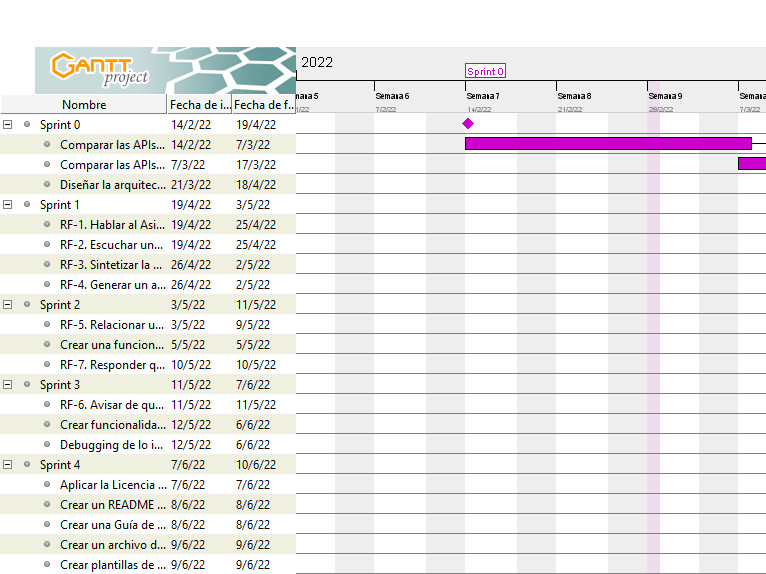
\includegraphics[width=\textwidth]{imagenes/GanttTR3.png} \\
	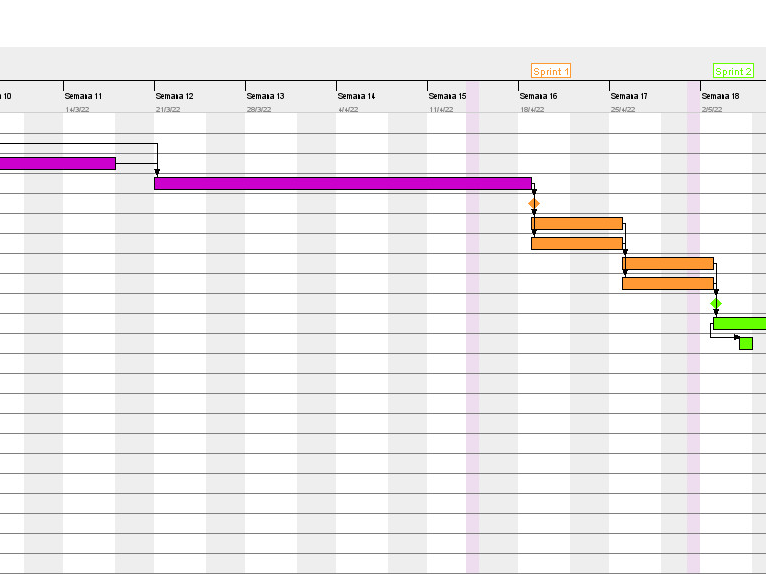
\includegraphics[width=0.48\textwidth]{imagenes/GanttTR2.png}
	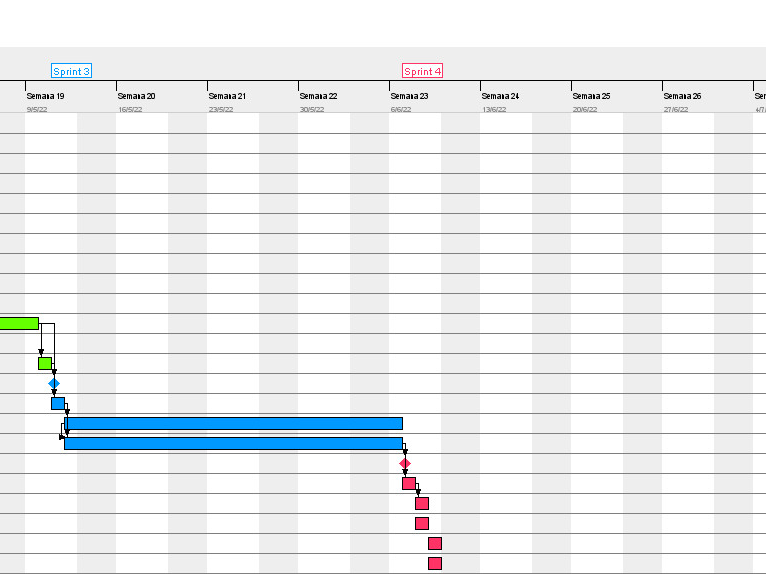
\includegraphics[width=0.48\textwidth]{imagenes/GanttTR1.png}
	\caption[Diagrama de Gantt]{Diagrama de Gantt del proyecto con los tiempos reales. De elaboración propia, generado con GanttProject.}
	\label{fig:gantt_tr}
\end{figure}

\subsection{Cumplimiento de los objetivos}

Durante el desarrollo se han tratado de cubrir los objetivos tanto de Investigación y Aprendizaje como de Diseño y Desarrollo.

\subsubsection{Objetivos de Investigación y Aprendizaje}

\begin{enumerate}[O-{IA}.1 -]
	\item Entender el funcionamiento de los Asistentes de Voz. (100\% completado.)
	\item Analizar el panorama del campo de los Asistentes de Voz y los avances que se han realizado.(100\% completado.)
	\item Analizar desde un punto de vista competitivo las prestaciones que ofrecen otras alternativas propietarias y libres (si las hay). (100\% completado.)
	\item Sintetizar los posibles componentes que conforman un Asistente de Voz y la escalabilidad de cada uno de ellos. (100\% completado.)
	\item Entender el impacto del software propietario y sus alternativas libres o de Código Abierto. (100\% completado.)
	\item Analizar las distintas licencias que se ofrecen y las compatibilidades entre éstas para elegir la idónea para la aplicación resultante. (100\% completado.)
	\item Leer sobre aquellos estándares y convenciones para facilitar la compartición y liberación del proyecto (por ejemplo. Códigos de conducta, Guías de contribución) (100\% completado.)
	\item Analizar el impacto que los descubrimientos en los Asistentes de Voz pueden producir en la Sociedad de la Información. (100\% completado.)
\end{enumerate}

\subsubsection{Objetivos de Diseño y Desarrollo}

\begin{enumerate}[O-DD.1 -]
	\item Diseñar personas y casos de uso en los que el software podría presentar algún problema con tal de buscar soluciones o limitaciones. (100\% completado.)
	\item Diseñar las clases que albergarán los componentes de un Asistente de Voz, su interacción con los periféricos de Entrada/Salida y con aquellas APIs externas que se requieran para el funcionamiento básico del programa. (100\% completado.)
	\item Idear una vía para escalar el número de posibles frases e interacciones que pueda reconocer el proyecto. (100\% completado.)
	\item Planear la arquitectura del proyecto resultante, siguiendo las buenas prácticas del Desarrollo de Software. (100\% completado.)
	\item Con base a la arquitectura, codificar lo necesario para la implementación de la aplicación. (100\% completado.)
	\item Redactar documentación referida a la arquitectura del proyecto para su posterior mantenimiento y escalabilidad. (100\% completado.)
	
\end{enumerate}


\section{¿Y ahora qué? Posibles trabajos y mejoras en el futuro.}
Si bien el proyecto puede ser usable y se le podría dar el \textit{status} de Producto Mínimo Viable, hay algunas cuestiones que facilitarían el uso y desarrollo de Arcadia para otros desarrolladores, o son tareas que no se han podido realizar durante el desarrollo. Listaremos algunos de ellos:

\begin{itemize}
	\item Los listados en la sección \ref{sect:unfinished-dev}, a los que estaría bien echar otro vistazo y acotarlos desde otro punto de vista.
	\item Añadir elementos de Integración Continua y Despliegue Continuo. Esto podría ayudar a automatizar los procesos monótonos como el formato del código, o ayudar a otros desarrolladores a subir su código según los estándares. Para ello, se estudiará sobre el tema y se tratará de integrar estos procesos a través de la forja usando GitHub Actions.
	\item Mejorar la documentación, tanto la calidad de este (añadiendo guías para realizar algunos cambios, por ejemplo), como el formato de presentación (usando GitHub Pages  o creando una documentación en PDF, como alternativas).
\end{itemize}

\section{Arcadia, los Asistentes Virtuales y el impacto en la sociedad}
Como se comentó en la Introducción, estamos en una época donde las nuevas tecnologías tratan de ser explotadas rápidamente, conectando a las personas y la información que se puede generar de ellas para propósitos variados. Además se habló de cómo las empresas protegían sus intereses y las protecciones que el estado les ofrece, y cómo el Software Libre y el Software de Código Abierto pueden resultar como alternativas de tal modelo proteccionista.

Los Asistentes Virtuales, como ejemplo de tecnología recientemente puesto a explotación por grandes empresas, son a veces objeto de sospechas por parte del público general y pueden causar cierto sentimiento de vigilancia. Aún así, la mayoría que usa ese tipo de aplicaciones tiende también a antropomorfizar la voz \cite{va-antromorfismos} que sale del altavoz, haciéndolo familiar. De esta forma, nos encontramos con una especie de limbo ético en este campo, ya que nos encontramos entre la usabilidad del producto, la demanda del público, y el interés de terceros por saber lo que una persona quiere o necesita.

Para resolver este problema, como hemos podido ver durante el transcurso de este Trabajo, se puede volver a pensar en estos sistemas con otros prismas. Uno de estos, el cual hemos explorado en detalle en este proyecto, es usar el Software Abierto y Libre y crear un núcleo que contenga esos proyectos, que se pueda adaptar a otras implementaciones y que todo lo que concierne a la aplicación se pueda consultar en cualquier momento gracias a que el código es público.

Teniendo en cuenta esta base, se ha tratado de conseguir que Arcadia cumpla con estas premisas, y que además sea abierto para cualquiera para hacer los cambios que desee, o reportar cualquier incidencia. De esta manera, la comunidad de desarrolladores y curiosos en la materia podrían ayudar a mantener la responsabilidad ética de este proyecto.

Aún así, se podrían dar algunas cuestiones que romperían los principios del proyecto. Al ser abierto, cualquiera podría hacer los cambios que desee, incluyendo la combinación del núcleo con un componente privativo, haciendo que esa versión alternativa no sea totalmente libre. Aún así, debido a que nuestro software está regido por la licencia AGPLv3 \cite{gplv3}, tiene en regencia las 4 Libertades \cite{fsf-philosophy}, de las cuales las 3 últimas permiten esa copia y redistribución.

Por otra parte, al ser un núcleo del que se conectan otros proyectos, podemos tener como preocupación el soporte de esos componentes. Puede que con el tiempo, esos componentes pasen a ser obsoletos y/o dejen de usar licencias compatibles con la que tiene Arcadia. De todas formas, gracias a la forma para realizar las adaptaciones, podemos introducir otros proyectos al software, formando así muchos sabores y versiones de esta aplicación, y pudiendo paliar así el problema.

\section{El proceso de aprendizaje y la distribución del conocimiento}
Desde la redacción de la primera página, se ha realizado un proceso de aprendizaje pautado sobre los conceptos a desarrollar y en qué fundamentos se basaban las tecnologías de los componentes a usar, para después buscar alternativas que utilizar en base a los intereses y restricciones del proyecto, y finalmente evaluarlos y usarlos para la codificación de Arcadia. En el proceso se han consultado multitud de portales web, papers y algún que otro manual o portal de documentación. En especial, se podría destacar la documentación de Rasa, ya que era muy completa y describía cualquier detalle relacionado con el entorno, con un portal de documentación web y muchas videoguías que permitieron probar el software y aprender a hacer funcionalidades sin mucha dificultad.

Aunque se ha querido explicar todo en esta Memoria, puede que haya un público muy reducido que acabe leyéndola (aunque esté disponible en GitHub), por lo que se ha querido también exponer este aprendizaje a cualquier interesado. De esta manera se realizó una charla en Marzo de 2022 hablando sobre los componentes de un Asistente Virtual y experimentando su funcionamiento. A pesar de los errores técnicos y la inexperiencia dando este tipo de exposiciones, los asistentes llegaron a comentar que les interesó mucho.



\section{Unas últimas palabras: Valoración personal}
Para esta sección, permitidme que pase de la tercera a la primera persona para poder contar las sensaciones y valoraciones que tengo en estas últimas líneas de la Memoria.

Hacer este trabajo ha sido la mezcla de un interés que tenía latente desde la mitad del transcurso de la carrera; junto con la necesidad de hacer un Trabajo Final de Grado que pudiera ser interesante y que permitiera plasmar todo lo aprendido durante esta etapa y cerrarla con satisfacción.

Han pasado aproximadamente 7 meses desde la primera reunión con el Tutor del TFG donde se discutieron las ideas escritas en un correo que recogía la propuesta, y gracias a lo cual se pudo definir todo el rumbo que llevaría este proyecto. Desde entonces, el flujo de correos y reuniones para revisar cómo iba esta aplicación ha sido llevadero y ameno, donde las correcciones y apreciaciones me servían para poder mejorar la redacción y los contenidos que quería exponer en este escrito. 

Desarrollar a Arcadia ha sido una pequeña odisea que ha requerido un tiempo considerable, pero se ha podido conllevar bien con el resto de tareas académicas, profesionales y personales. También me ha servido de desafío personal para ser constante y mejorar y aplicar todo lo acontecido en la etapa universitaria.

Si bien este proyecto no deja de ser un Trabajo Final de Grado, desearía continuar con el desarrollo de este. Quizás como hobby, como distracción o como manera de aplicar nuevas tecnologías relacionadas. 

Aprender por cuenta de uno mismo tiende a ser un paso natural en este tipo de trabajos, pero a pesar de ello siempre viene bien toda ayuda (sea a través de material o hablando con alguien que sepa de alguno de los temas que rodeen lo que se quiere saber). Por mi parte, sentía también que una parte de aprender es enseñar a otros que les interesen, dando pie a un ciclo virtuoso.

En definitiva, y dando punto y final a esta Memoria, ha sido un TFG que he disfrutado en la confección y donde me he sentido bien asesorado y capacitado para cumplir con lo descrito, cosa que puede que continúe realizando y enseñando en el futuro.
